\chapter{Vacuum polarization}
\label{cha:Vacuum-Polarization}

\section{The setup}
%\note{This first order backreaction calculation should only be valid up to $\varepsilon \lambda \ll 1$ (?). In the problem of a charged particle of charge $e$ colliding with a nucleus of charge $Ze$, vacuum polarization becomes relevant when the coupling constant becomes comparable to the source. Where to discuss this? What when this approximation isn't true?}

We study the coupling of a massive charged (complex) scalar field $\phi$ to the electromagnetic field $A_\mu$ in the presence of a background generated by external sources $j^\mu_\text{C}$. This is described by the Klein-Gordon-Maxwell action
\begin{align}
	S_{KGM} [\phi, A_\mu] = \int_{\mathbb{R}^2}^{} dx^{0}dx^{1} \left( D_\mu \phi D^*{}^{\mu}\phi^* 
	+ m^2\phi^* \phi - \frac{1}{4}F_{\mu\nu} F^{\mu\nu} + A_\mu j_{\text{C}}^{\mu} \right)  	
	\label{eq:KGM-action}
\end{align}
with $D_\mu = \partial_\mu + ieA_\mu$ the gauge covariant derivative given by the minimal coupling to $A_\mu$ and  $e$, $m$ the charge and mass of the Klein-Gordon field, respectively. $F_{\mu\nu} = \partial_\mu A_\nu - \partial_\nu A_\mu$ is the electromagnetic stress-energy tensor and $j_{\text{C}}^\mu$ is a conserved charge current determining the external electromagnetic field.

Variation of the action \eqref{eq:KGM-action} with respect to $\phi$, $A_\mu$ yields the Klein-Gordon-Maxwell equations, namely the coupling of the Klein-Gordon and the Maxwell equations, 
\begin{subequations}
	\begin{align}
			\left( D_\mu D^\mu +m^2  \right) \phi = 0 
		\label{eq:klein-gordon-equation}\\
			\partial_\mu F^{\mu\nu}= j_{\text{C}}^{\nu} + j_{\text{br}}^\nu 
		\label{eq:quantum-maxwell-equation}
	\end{align}
\end{subequations}
with 
\begin{align}
	j^{\nu}_{\text{br}} = ie\left( \phi^* D^\nu \phi - \phi D^\nu^* \phi^* \right) 
\end{align}
the charge current density of the Klein-Gordon field. 

We study however the semi-classical approximation, in which the quantum field propagates in a classical background, and it acts as a source for the electromagnetic field through its expectation value with respect to some state, in this case the vacuum. This approximation is said to hold when the charges are not too strong. In Quantum Electrodynamics in 4 spacetime  dimensions this limit is usually set to the Schwinger limit $E_\text{crit} \sim \frac{m_e^2}{e}$ \cite{Schw51}, beyond which the non-linear behavior of the vacuum can no longer be ignored.

In this approximation, $\phi$ propagates under the influence of a classical electromagnetic field, and the source of the latter is modeled as follows
\begin{subequations}
\begin{align}
            ((\partial_\mu + ieA_\mu(t, x)) (\partial^\mu + ieA^\mu(t, x)) + m^2)\phi = 0 \\
			\partial_\mu F^{\mu\nu}= \partial_\mu \partial^\mu A^\nu -  \partial_\mu \partial^\nu A^\mu  = j_{\text{external}}^{\nu} + \left<j_\text{br}^{\nu} \right>_\omega.
			\label{eq:semi-classical-maxwell}
\end{align}
\end{subequations}
Here, $\omega$ is the state of $\phi$ with respect to which the expectation value $\left<j_\text{br}^{\nu} \right>_\omega$ is taken.
We look for the solutions $A_0$ and $\omega$ of the semiclassical Klein-Gordon-Maxwell equations. 
\note{Take a look at this}

In this work, we study the region $x\in[0,a]$, delimited by two charged $q, -q$ placed at the left and right boundaries, respectively. This generates a constant, time-independent electric field of strength $E=q$ which points towards positive $x$.
There is freedom in the choice of the boundary conditions for the Klein-Gordon equation, namely, Dirichlet $\left. \phi\right|_{x^1 = 0, a}=0$  or Neumann $\left. \partial_{1}\phi\right|_{x^1 = 0, a}=0$ boundary conditions\footnote{The more general Robin boundary conditions can be applied, but they will not be studied in the current work. An example of boundary conditions to avoid are periodic, as a traveling particle would get accelerated as it traverses the interval and is influenced by the electric field $E$.}. However, equation \eqref{eq:semi-classical-maxwell} needs to be solved with specific boundary conditions, so that the electric field at the boundaries is precisely $q$ and no screening is observed.

%The Maxwell equations read 
%\begin{align}
%	\begin{split}
%		\partial_\mu \partial^\mu A^{0}- \partial_\mu \partial^0 A^{\mu} &= \rho \\
%		\partial_\mu \partial^\mu A^{1}- \partial_\mu \partial^1 A^{\mu} &= 0
%	\end{split}
%\end{align}
We choose the Coulomb gauge $\partial_1 A_1 = 0$, under which
 $A_1$ can be set to 0, and $A_0$ solves the Poisson equation 
\begin{align}
	 \partial_1^2 A_0 = -\rho
	 \label{eq:poisson}
\end{align}
in the region $x^1 \in (0, 1)$.
The only external charges we consider in this setup are those sitting at the boundaries $x=0, a$. In the region between them, $\rho$ is only made up of the contribution from the vacuum polarization, and in solving Equation \eqref{eq:poisson} we treat the boundary charges as the boundary conditions, 
%%Equation \eqref{eq:poisson} to be solved with 
\begin{align}
 	  \left.\partial_1 A_0 \right|_{x_1=0, a}=-q,
		  \label{eq:boundary-conditions-A0}
\end{align}
so that close to the boundaries, the vacuum polarization does not screen the boundary charges and the measured charge by Gauß's theorem is $q$.
This amounts to solving the Poisson equation with Neumann boundary conditions, the solution of which is unique up to an addition constant (c.f. section 1.9 of \cite{Jackson:1998nia}), which is  conveniently chosen such that $A_0$ is antisymmetric 
on $[0, 1]$. It suffices to demand $A_0(\frac{a}{2}) = 0$. 
Equation \eqref{eq:poisson} is solved by 
\begin{align}
\begin{split}
			A_0(x^{1}) =
				   -q\left( x^{1}-\frac{a}{2} \right) - \int_{\frac{a}{2}}^{x^{1}}\int_{0}^{x^{1}'}     \rho(x^{1}'') dx^{1}'' dx^{1}' .
                   \label{eq:A0-full}
\end{split}
\end{align}

In the chosen gauge, the Klein-Gordon equations take the form
\begin{align}
    \left( -(\partial_0 +ie A_0(x^{1}))^2 + \partial_1^2 + m^2 \right) \phi = 0.
    \label{eq:TDKGE}
\end{align}

Finally, defining the dimensionless parameters 
		\begin{align}
			\begin{split}
				(t, z) &= \left(\frac{x^{0}}{a}	,\frac{x^{1}}{a}	  \right) \\
					\lambda = ea^2q,  \hspace{0.5cm}
				\varepsilon &= ae, \hspace{0.5cm}
				\omega_n = a\Omega_{n},
%				\lambda &= ea^2E \\
%				\varepsilon &= ae \\
%				m &= a\mu \\
%				\omega_n &= a\Omega_n,
			\end{split}
		\end{align}
		and using the ansatz
		$	\phi(t, z) = \phi_n(z) e^{-i\omega_n t},$
		allows us to split \eqref{eq:TDKGE} into the dimensionless mode equations 
		\begin{align}
			\left( (\omega_n - \varepsilon A_0(z) )^2 + \frac{d^2}{dz^2}- a^2m^2 \right) \phi_n(z) = 0.
		\label{eq:TIKGE}
		\end{align}
		Each of the modes is normalised with respect to the inner product
		\begin{align}
			(\phi_n, \phi_m) = i \int_{0}^{1} dz \left( \pi^*_n \phi^*_m - \pi_m \phi_n \right),
			\label{eq:symplectic-inner-product}
		\end{align}
		with $\pi_n^* = D_0\phi_n$ the canonical conjugate of $\phi.$ Positive (negative) energy solutions are normalized to $+1$ ($-1$).

		\section{Quantization and vacuum polarization}

		Following the canonical quantization procedure laid out in the Section \ref{sec:quantization}, 
		\begin{align}
			\phi(t, z) = \sum_{n>0}^{} a_n \phi_n(z) e^{-i\omega_n t} + \sum_{n<0}^{} b_n^\dagger \phi_n(z) e^{-i\omega_n t},
		\end{align}
		with $a_n, a_n^\dagger$ and $b_n, b_n^\dagger$ the ladder operators for the positive and negative energy solutions, respectively. The $n>0$ and $n<0$ solutions correspond to positive and negative norm single frequency solutions $\phi_n(z) e^{-i\omega_n t}$, respectively
         Furthermore, the antisymmetry of $A_0$, implies  $\omega_{-n} = -\omega_n$ allowing as to identify positive (negative) norms with positive (negative) energies\footnote{Global gauge transformations,  $A_0 \to A_0 + \xi$, shift the spectrum as $\Omega_n \to \Omega_n + e\xi$,  and thus $\Omega_{-n} \neq -\Omega_n$, but defining $\omega_n = a\Omega_n -  \varepsilon \xi$ ensures the invariance under global gauge transformations of $\omega$ and thus $\omega_{-n} = -\omega_n$.}.
        
		The vacuum polarization of the Klein-Gordon field
		\begin{align}
			\rho(z) = i\varepsilon \vacuum{ \phi^* D_0\phi(z) - \phi D_0^* \phi^*(z) }.
			\label{eq:vacuum-polarization}
		\end{align}
        is a priori ill-defined due to the distributional nature of $\phi$.
        We define $\rho$ through point-splitting renormalization with respect to a Hadamard parametrix by Equation \eqref{eq:point-splitting-wrt-a-Hadamard-parametrix}, as was explained in the section \ref{sec:Hadamard}.
        
		The Hadamard parametrix $H^{\phi^*\phi}(x, x') $ of the Klein-Gordon field in 1+1 dimensions up to relevant order\footnote{The charge density operator only has first order derivatives, and therefore higher orders in the Hadamard parametrix will vanish after taking the limit $x'\to x$ }
        is given by
		\begin{align}
			H^{\phi^* \phi}(x, x') = -\frac{1}{4\pi}V_0(x, x') \log (-(x-x')^2_\varepsilon).
		\end{align}

	The smooth coefficient $V_0(x, x')$  is calculated in \cite{Schl2015} as a solution to the transport equation \eqref{eq:transport-equation}
	\begin{align}
		V_0(x, x') = \exp \left( -i\varepsilon \int_{0}^{1} A_\mu(x' + s(x-x')) \left( x- x' \right) ^{ \mu} ds  \right),
	\end{align}
    which corresponds to the parallel transport along the straight line joining the points $x$, $x'$.
	In the chosen gauge $A_\mu(t, z) = (A_0(z), 0)$, and performing the point-splitting in the time direction, $x' =  (t+\tau, z)$, 
	\begin{align}
	V_0(z, t; z,t+\tau ) = \exp\left( -i\varepsilon\tau A_0(z) \right).
	\end{align}
    To avoid cluttering of notation, the $z$ dependence is henceforth dropped.

We calculate the vacuum expectation value of the first term in equation \eqref{eq:vacuum-polarization}.  In this point-splitting, the two-point function  $w_0^{\phi^*\phi }(x, x')$ takes the form
	\begin{align}
		w_0^{\phi^* \phi}(x, x') = \vacuum{\phi^*(x) \phi(x')} = \sum_{n<0}^{} \abs{\phi_n}^2 e^{-i \omega_n \left( \tau + i\epsilon \right) },
	\end{align}
where an $i \epsilon$-prescription is used in order to ensure convergence. In view of Equation \eqref{eq:point-splitting-wrt-a-Hadamard-parametrix}, we calculate 
\begin{align}
	D_0'w^{\phi^* \phi}(x, x') &= -i \sum_{n<0} (\omega_n - \varepsilon A_0)\lvert \phi_n \rvert ^2 e^{-i\omega_n (\tau+i\epsilon)},
\end{align}
and 
\begin{align}
	D_0' H^{\phi^*\phi}(x, x') &= -\frac{1}{2\pi}\frac{1}{\tau + i\epsilon} - \frac{i\varepsilon A_0 }{2\pi} + \mathcal{O}(\tau).
\end{align}
This implies 
\begin{align}
\begin{split}
\vacuum{  \phi^* D_0\phi(x)}  = -i\lim_{\tau \to 0} 
 &\left[\sum_{n<0}^{} (\omega_n - \varepsilon A_0)\abs{\phi_n}^2 e^{-i \omega_n \left( \tau + i\epsilon \right) } \right.\\
& \hspace{1.5cm}\left.+\frac{1}{2\pi}\frac{1}{\tau + i\epsilon} \right]- \frac{i\varepsilon A_0 }{2\pi} 
\end{split}\end{align}

Similarly, for the second term in \eqref{eq:vacuum-polarization}, 
\begin{align}
	D_0^*'w^{\phi\phi^* }(x, x') &= i \sum_{n>0} (\omega_n - \varepsilon A_0)\lvert \phi_n \rvert ^2 e^{i\omega_n (\tau+i\epsilon)},
\end{align}
and
\begin{align}
	D_0^*' H^{\phi\phi^*}(x, x') &= -\frac{1}{2\pi}\frac{1}{\tau + i\epsilon} + \frac{i\varepsilon A_0 }{2\pi} + \mathcal{O}(\tau),
\end{align}
since $V_0(x, x')^* = V_0(x', x)$.
This implies 
\begin{align}
\begin{split}
\vacuum{  \phi(x)D_0\phi(x)^* }  = i\lim_{\tau \to 0} 
 \left[\sum_{n>0}^{} (\omega_n - \varepsilon A_0)\abs{\phi_n}^2 e^{i \omega_n \left( \tau + i\epsilon \right) }\right.
\\\left.+\frac{1}{2\pi}\frac{1}{\tau + i\epsilon} \right]- \frac{i\varepsilon A_0 }{2\pi} 
\end{split}\end{align}

When substituting into Equation \eqref{eq:vacuum-polarization}, the divergent terms cancel out, resulting in the well-defined expression for the renormalized vacuum polarization 
\begin{align}
	\begin{split}
			&\rho(z) =  \\
			&\varepsilon\lim_{\tau \to 0}\left(
			\sum_{n< 0}^{} (\omega_n - \varepsilon A_0) \lvert\phi_n\rvert^2 e^{-i \omega_n (\tau + i\epsilon)}  +
			\sum_{n> 0}^{} (\omega_n - \varepsilon A_0) \lvert\phi_n\rvert^2 e^{i \omega_n (\tau + i\epsilon)}  \right)
			+ \frac{\varepsilon^2}{\pi} A_0.
	\end{split}
	\label{eq:Hadamard-vacuum-polarization}
\end{align}

\cite{Ambj1983} calculate the vacuum polarization by defining the contribution of each of the modes to the total charge density
\begin{align}
    \rho_n (z) = 2 \varepsilon (\omega_n - \varepsilon A_0(z)) \lvert \phi_n(z)\rvert ^2,
\end{align}
 The vacuum polarization is calculated by pairing the positive and negative norm solutions 
\begin{align}
\rho(z) = \frac{1}{2}\sum_{n>0}\left( \rho_n(z) + \rho_{-n}(z)\right)
\end{align}
which is ill-defined as it relies on the pairing of the modes in the series in order to be convergent. This expression presents two main differences with Equation \eqref{eq:Hadamard-vacuum-polarization}, the lacking of the exponentials $e^{i\omega_n (\tau + i \epsilon)}$ inside of the limit as a consequence of taking the coinciding points limit, and the extra $\frac{\varepsilon^2}{\pi} A_0$ term.

\note{I do not like the writing of this paragraph}

\section{The external field approximation}
To study the relevance of the backreaction of the scalar field we first study the external field approximation, ignoring the backreaction of the scalar field. In this approximation, $\varepsilon A_0(z) = -\lambda \left( z-\frac{1}{2} \right) $, and therefore equation \eqref{eq:TIKGE} takes the form
		\begin{align}
			\left( \left[(\omega_n + \lambda\left( z-\frac{1}{2} \right)\right] ^2 + \frac{d^2}{dz^2} - a^2m^2 \right) \phi_n = 0.
			\label{eq:klein-gordon-in-the-external-field-approximation}
		\end{align}

		With the appropriate parameter definitions, 
		\begin{align}
			x = \frac{1+i}{\sqrt{\lambda} } \left[ \omega_n + \lambda \left(z - \frac{1}{2}\right) \right] , \,\,\,\,\,\, n = -\frac{a^2m^2}{2\lambda} - \frac{1}{2},
		\end{align}
		equation \eqref{eq:klein-gordon-in-the-external-field-approximation}  can be identified with the Weber equation 
		\begin{align}
			 \frac{d^2 D_n(x)}{dx^2} + \left(n+ \frac{1}{2 }-\frac{1}{4}x^2\right) D_n(x) = 0,
			 \label{eq:Weber-equation}
		\end{align}
		which is solved by the parabolyc cylinder functions $D_n(x)$ defined in \cite{Whittaker_Watson_1996}.
		The general solution to Equation \eqref{eq:klein-gordon-in-the-external-field-approximation} is written as
\begin{align}
	\begin{split}
	\phi_n(z) &= 
	a_n D_{i \frac{m^2a^2}{2\lambda} - \frac{1}{2}} \left( 
		\frac{1+i}{\sqrt{\lambda} }
		\left( \omega_n + \lambda \left( z-\frac{1}{2} \right)
		\right) 
	\right)  \\
	&+
	b_n D_{-i \frac{m^2 a^2}{2\lambda} - \frac{1}{2}} \left( 
		\frac{i - 1}{\sqrt{\lambda} }
		\left( \omega_n + \lambda \left( z-\frac{1}{2} \right)
		\right) 
	\right),
	\end{split}
	\label{eq:parabolyc-cylinder}
\end{align}
where the parameters $\omega_n, a_n, b_n$ are to be calculated by applying the corresponding boundary and normalization conditions for the field $\phi_n$.


However, this model presents an instability in the sense that when increasing the external electric field strength $\lambda$ past a certain critical value $\lambda_c$, the vacuum polarization diverges and the energy of the modes goes into the complex realm. This leads to runaway solutions, as the complex exponentials  $e^{i \omega_n t }$ turn into real exponentials (\cite{Ambj1983}). The appearance of this instability is shown in Figure \ref{fig:figures-eigenvalues-external-field-approximation-png}, where the energy of the first mode is represented, as $\lambda$ approaches $\lambda_c$. 

\begin{figure}[t]
	\centering
	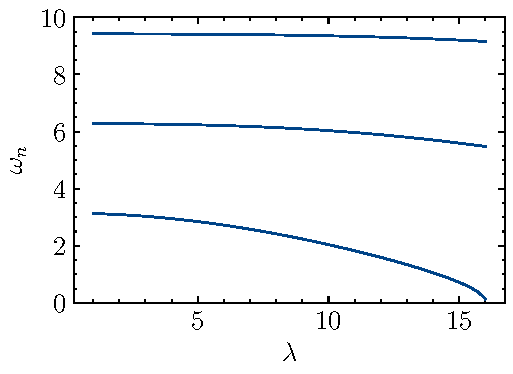
\includegraphics[width=1\textwidth]{figures/dirichlet/eigenvaluesExternalFieldApproximation.pdf}
\caption{The energy of the first three modes of $\phi$ as the background electric field strength $\lambda$ is increased, illustrating the vertical drop to 0 when $\lambda\to \lambda_c$, which displays the emergence of the critical $\lambda$.}
	\label{fig:figures-eigenvalues-external-field-approximation-png}
\end{figure}

\cite{Ambj1983} claim that the screening nature of the Klein-Gordon vacuum is enough to raise the energy of the modes enough in order to avoid these instabilities. However, the vacuum polarization in \cite{Ambj1983} is not calculated properly \cite{Wernersson2020}. As we state in the following section, the back-reaction of the Klein-Gordon field, as wrongly calculated by \cite{Ambj1983} is much stronger than the one calculated in \cite{Wernersson2020}. This raises the question to be answered in this Thesis: 
\begin{center}
    \textbf{Under the correct renormalization procedure, is the back-reaction of the Klein-Gordon field strong enough so as to avoid the instabilities found when $\lambda > \lambda_c$?}
\end{center}

\subsection{Perturbative approximation}

%Following the steps of \cite{Ambjorn1983, Wernersson2020}
%, it might be instructive to study the problem perturbatively. We state the problem as a Schrödinger-like equation 
%\begin{align}
%	i \partial_t \ket{\Psi} = H \ket{\Psi}
%	\label{eq:schrodinger}
%\end{align}
%with 
%\begin{align}
%	\ket{\Psi} = \begin{pmatrix} \phi \\ \pi^* \end{pmatrix}, 
%\text{and }\pi^* = D_0 \phi.
%\end{align}
%The space of all $\ket{\Psi}$ equipped with the inner product  \eqref{eq:symplectic-inner-product} forms the phase space of our system.
%
%We can construct the corresponding Hamiltonian operator as 
%\begin{align}
%	H= i \begin{pmatrix} 
%	0 & 1 \\
%	D_1 ^2 - m^2 & 0
%\end{pmatrix}
%+ \begin{pmatrix}  
%	eA_0 & 0 \\
%	0 & eA_0
%\end{pmatrix} 
% = H_0 + H_1.
%\end{align}
%The Hamiltonian $H$ is split into a free field hamiltonian $H_0$ and consider $H_1$ to be a perturbation. $H$ is hermitean with respect to the inner product \eqref{eq:symplectic-inner-product}.
%The eigenstates $\Psi_n$ of $H_0$ with eigenvalues $\omega_n$ are the solutions to a free particle in a box  f size 1. For Dirichlet boundary conditions ($\Psi(0) = \Psi(1) = 0$),
%\begin{align}
%	\omega_n^D = \text{sign}(n) \sqrt{m^2 + \pi^2 n^2} ,\hspace{1cm} \phi_n^D(z) = \lvert \omega_n \rvert ^{-\frac{1}{2}} \sin \pi n z,
%	\hspace{0.3cm}	n \in \mathbb{Z} \setminus \{0\} ,
%\end{align}
%For Neumann boundary conditions $(\Psi'(0) = \Psi'(1) = 0)$ one has 
%\begin{align}
%	\omega_{n \neq 0}^N = \text{sign}(n) \sqrt{m^2 + \pi^2 n ^2},
%	\hspace{0.4cm}	& \phi^N_{n\neq 0} (z) = \lvert \omega_n \rvert ^{- \frac{1}{2}}\cos \pi n z \\
%	\omega_{\pm 0}^N = \pm m,
%	\hspace{0.4cm}	& \phi^N_{\pm 0} (z) = \left( 2m \right) ^{-\frac{1}{2}}.
%\end{align}
%These eigenstates are the zeroth order correction $\ket{\Psi_n^{(0)}}$ to the $H_0$ eigenstates. The first order correction is given by perturbation theory  
%\begin{align}
%	\omega_n ^{(1)} &= \frac{\bra{\Psi_n^{(1)}}\ket{H_1\Psi_n^{(1)}}}{\bra{\Psi_n^{(0)}}\ket{\Psi_n^{(0)}}} \\
%	\ket{\Psi_n ^{(1)}} &= \sum_{k\neq n}^{} 
%	\frac{
%		1
%	}
%	{
%	\bra{\Psi_n^{(0)}}\ket{\Psi_n^{(0)}}
%	}
%	\frac{
%	\bra{\Psi_k^{(0)}}\ket{H_1\Psi_n^{(0)}}
%	}{
%	\omega_n ^{0} - \omega_k^{(0)}
%	} \ket{\Psi_k^{(0)}}
%\end{align}

It might be enlightening to see the mode solutions and vacuum polarization at first perturbative order. These calculations were already done in \cite{Ambj1983, Wernersson2020}, and we therefore just state the perturbative corrections to the free field solutions, for Dirichlet boundary conditions (marked with a superscript D) and for Neumann boundary conditions (marked with a superscript N). 
\begin{align}
	\begin{split}
	\phi_n^{D} &= \left( m^2 + \pi^2  n^2 \right)^{-\frac{1}{2}} \Biggl[ \sin\pi n z \\
		   &\left.+ \lambda \frac{\sqrt{m^2 + \pi^2 n^2} }{2 \pi \lvert n \rvert} 
		\left( 
		\frac{1}{\pi n}\left( \frac{1}{2} - z \right) \sin \pi n z - z(1-z) \cos \pi n z \right) 
	\right] 
	\end{split} 
	\label{eq:perturbative-dirichlet}
	\\
	\begin{split}
	\phi_n^{N} &= \left( m^2 + \pi^2 n^2 \right)^{-\frac{1}{2}} 
	\Biggl[ \cos\pi n z   \\
		   &\left. + \lambda \frac{\sqrt{m^2 + \pi^2 n^2} }{2 \pi \lvert n \rvert} 
		\left( 
		\frac{1}{\pi n}\left( \frac{1}{2} - z \right) \cos \pi n z 
	+ ( z(1-z) + (\pi n)^{-2)} ) \sin \pi n z \right) 
	\right] 
	\end{split}
	\label{eq:perturbative-neumann}
	\\
	\begin{split}
	\phi_{\pm 0 }^{N} &= \left( 2m \right) ^{- \frac{1}{2}} \mp \lambda \sqrt{2m} \left( \frac{1}{24} - \frac{1}{4}z^2 + \frac{1}{6}z^3\right).
	\end{split}
	\label{eq:perturbative-neumann-n-0}
\end{align}

These expressions for the mode solutions of the field can be used to calculate $\rho$ at first order in $\lambda$ using Equation \eqref{eq:Hadamard-vacuum-polarization}. We restrict ourselves to Dirichlet boundary conditions, and from now on drop the superscript D.
\begin{align}
\rho(z) = \varepsilon \lim_{\tau\to 0} \sum_{n=1}^{\infty} \left(  (\pi n - \varepsilon A_0)\lvert \phi_n\rvert ^2 -  (\pi n + \varepsilon A_0)\lvert \phi_{-n}\rvert ^2 \right)  e^{i \pi n (\tau + i \epsilon)} + \frac{\varepsilon^2}{\pi}A_0.
\label{eq:perturbative-vacuum-polarization}
\end{align}

From \eqref{eq:perturbative-dirichlet}, up to first order in $\lambda$,
\begin{align}
	\lvert \phi_n\rvert ^2 = \frac{1}{\pi\abs{n}} \left( \sin^2\pi n z - \lambda \sin\pi n z \left[ \frac{1}{\pi n } \left( z - \frac{1}{2} \right) \sin \pi n z + z (1- z) \cos \pi n z\right]  \right) .
\end{align}
Substituting in \eqref{eq:perturbative-vacuum-polarization}, and with some rearranging, 
\begin{align}
	\begin{split}
		\rho(z) &= -2\varepsilon \lambda \lim_{\tau \to 0} \sum_{n=1}^{\infty} z(1-z) \sin \pi n z  \cos \pi nz - \frac{\varepsilon \lambda}{\pi} \left( z-\frac{1}{2} \right) \\
		&= -\varepsilon\lambda  z(1-z) \lim_{\tau \to 0} \frac{1}{2i} 
		\left(
			\frac{e^{i \pi (2 z + \tau + i\epsilon)}}{1 - e^{i\pi( 2z + \tau + i\epsilon) }} 
			- \frac{e^{i \pi (-2 z + \tau + i\epsilon)}}{1 - e^{i\pi( -2z + \tau + i\epsilon) }} 
		\right) 
		- \frac{\varepsilon\lambda}{\pi} \left( z-\frac{1}{2} \right) \\
		&= -\varepsilon \lambda  \frac{z(1-z)}{2} \cot \pi z	- \frac{\varepsilon\lambda}{\pi} \left( z-\frac{1}{2} \right).
	\end{split}
\end{align}

In \cite{Ambj1983}, the vacuum polarization at first order in $\lambda$ has precisely the same expression,
\begin{align}
	\rho  =  -  \varepsilon\lambda \frac{z (1-z)}{2} \cot(\pi z),
\end{align}
with the additional potential term lacking.

\begin{figure}[t]
	\centering
	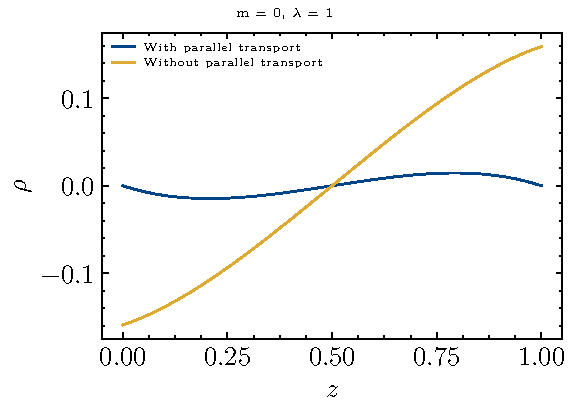
\includegraphics[width=0.8\textwidth]{figures/dirichlet/hambjorn.pdf}
	\caption{The vacuum polarization at first order in $\lambda$ in Dirichlet boundary conditions for the massless Klein-Gordon field. In orange, $\rho$ as calculated using the mode sum in \cite{Ambj1983}, and in blue using point splitting with respect to the Hadamard parametrix as in \cite{Wernersson2020}. }
	\label{fig:perturbative-rho-comparison}
\end{figure}
We show in the figure \ref{fig:perturbative-rho-comparison} the comparison between the two $\rho$. Notice how the addition of the potential term resulting from the parallel transport in \eqref{eq:Hadamard-vacuum-polarization} forces $\rho$ to be 0 at the boundaries, as one would expect for Dirichlet boundary conditions. 
\section{Self-consistent fields}

We study the solutions to the semi-classical Klein-Gordon-Maxwell equations in the presence of a background electric field strength $\lambda$ as an infinite dimensional fixed point problem (cf. Chapter 1 of \cite{Temam1997}), i.e.~the solutions $A_{0, \lambda}$ to the equation 
\begin{align}
    A_{0, \lambda} = f(A_{0, \lambda}).
    \label{eq:update-law}
\end{align}
In the present case, $f$ is a complicated function, which in summary
\begin{enumerate}
    \item calculates the solutions $\phi$ of Equation \eqref{eq:TIKGE} for the given $A_0$,
    \item calculates $\rho$ using Equation \eqref{eq:Hadamard-vacuum-polarization},
    \item returns $A_0$ calculated in Equation \eqref{eq:A0-full}.
\end{enumerate}
These solutions are looked for by studying $A_{0, \lambda}^\infty := \lim_{\kappa\to \infty}A_0^\kappa$, with $A_{0, \lambda}^\kappa$ the sequence of functions defined by successive applications of $f$:
\begin{align}
    A_{0, \lambda}^{\kappa+1} = f(A_{0, \lambda}^\kappa) = f^\kappa(A_{0, \lambda}^0),\hspace{0.4cm}f^k := \underbrace{f\circ ... \circ f}_{\kappa \text{ times}},
\end{align}
with $A_0^0$ the initial value for the potential, which for low $\lambda\ll \lambda_c$, can be safely taken to be the external field approximation
$$
\varepsilon A_{0, \lambda}^0(z) = -\lambda \left(z- \frac{1}{2}\right).
$$
The initial value $A_{0, \lambda}^0$ for higher values of $\lambda$ is discussed below in this section.

This sequence is expected to present oscillatory convergence, as for $\kappa=0$, the unscreened background electric field leads to a "strong vacuum polarization", and therefore "strong screening". The $\kappa=1$ "strongly screened" electric field leads to a "weak vacuum polarization". If the limit $\kappa\to\infty$ exists, one speaks of the self-consistent solutions to the semi-classical Klein-Gordon-Maxwell equation. We call $A_{0, \lambda}^\infty$ the self-consistent potential for $\lambda$.

At every iteration $\kappa$, the core steps in evaluating $f$ solve the equations
\begin{subequations}
\begin{align}
	\partial_1^2 \phi^{\kappa+1}_n &=
	\left( - (\omega^{\kappa+1}_n - \varepsilon A^{\kappa}_0)^2 + m^2 \right) \phi^{\kappa+1}_n
	\label{eq:iterative-TIKGE}\\
	\begin{split}
		\varepsilon A_0^{\kappa}(z) &= -\lambda\left( z-\frac{1}{2} \right)  - \varepsilon\int_{\frac{1}{2}}^{z} \int_{0}^{z'} \rho^{\kappa}(z'')  dz'' dz'\\
	\end{split}
	\label{eq:potential-at-step-kappa}
.
\end{align}
\end{subequations}
with $\rho$ calculated using \eqref{eq:Hadamard-vacuum-polarization}, up to a finite mode cutoff in the sum. This cutoff at mode N causes the calculated $\rho$ to be oscillatory, of period $\Delta z = \frac{1}{N+1}$, which is averaged out. 

When taking the limit $\kappa \to \infty$ following this procedure, we look for convergence of $A_{0, \lambda}$ in some norm $\norm{\cdot}$ defined by a \textit{relative} tolerance $\xi_\text{rel}>0$ such that when $\norm{A_{0, \lambda}^\kappa-A_{0, \lambda}^{\kappa-1}} < \xi_\text{rel} \norm{A_{0, \lambda}^{\kappa -1}}$ the iteration is halted and $A_{0, \lambda}^\infty =A_{0, \lambda}^\kappa $. 
\footnote{For convenience, we choose the $L_{\infty}$ norm $\norm{A_0}_{L_\infty} = \max(A_0)_{z\in [0,1]}$, which in our case coincides with $A_0(1)$. This is a consequence of the screening behavior of the vacuum. Other norms can be used, but one notices \textit{a posteriori} that for constant $m$, the induced $A_0^\text{br}$ are approximately proportional to one another (see e.g. Figure \ref{fig:different-lambda-rho}), and therefore changing the norm (e.g. $\norm{\cdot}_{L_1}$, $\norm{\cdot}_{L_2}$, \ldots) amounts to picking up overall constant factor which gets absorbed when studying the relative convergence of $A_0^\kappa$. 
} 

For higher $\lambda$ values, $A_{0, \lambda}^0 = -\lambda \left(z - \frac{1}{2}\right)$ is no longer a valid starting point, as $\lambda > \lambda_c$ no longer presents real $\omega_n$ in the external approximation \cite{Ambj1983}. 
When this is the case, the initial $A_{0, \lambda}^0$ should instead be the self-consistent $A_{0, \lambda'}^\infty$ calculated for a previous $\lambda'< \lambda$.  In this way, the algorithm for searching self-consistent solutions for different $\lambda$ values is constructed in the following manner:
\begin{enumerate}
    \item For a low enough $\lambda$\footnote{E.g. $\lambda=10$ in the massless case with Dirichlet boundary conditions, and $\lambda=0.1$ for $m=1$ with Neumann boundary conditions)}, set $A_{0, \lambda}^0(z) = -\lambda (z - \frac{1}{2})$.
    \item Try to calculate $A_{0, \lambda}^\infty$ through the procedure laid out above.
    \item If $A_{0, \lambda}^\infty$ exists, set $\lambda' = \lambda + \Delta \lambda$, with $\Delta\lambda>0$, and set $A_{0, \lambda+\Delta\lambda}^0=A_{0, \lambda}^\infty$.
    \item If, however, $A_{0, \lambda}^\infty$ could not be found\footnote{This can happen for two reasons: Either the $\lambda$ considered was big enough that the system could not find a solution (due to an electric field that is too strong to try to solve for without the corresponding screening due to the backreaction), or it did not converge. 
   % In the context of fixed point problems in 1 dimension an example of non-convergence is that of 
    }, set a smaller $\lambda$ and $\Delta \lambda$, and repeat step 1. 
\end{enumerate}
%once the self-consistent $A_{0, \lambda}$ is found for a low enough $\lambda$ which admits the external field approximation as an initial guess, in applying this scheme for a different $\lambda'>\lambda$, $A_{0, \lambda'}^0 = A_0^0$.
%Once a self-consistent solution is found, we use this solution as a guess for some new $\lambda'>\lambda$. In this way, we sample the whole $\lambda$-parameter space to study the interaction between the scalar field and the external electric field. 
For $\lambda \gtrsim \lambda_c$, the required $\Delta \lambda$ such that $A_{0, \lambda}^\infty$ exists decreases very quickly, as the effect of the backreaction gets increasingly relevant. It can get down to $\Delta \lambda \sim 10^{-7}$, which at around 30 seconds per $\lambda$ value amounts to approximately 10 years to achieve steps of unit size in $\lambda$.

To overcome this, we slightly modify the iterative procedure with a "relaxing" procedure, 
\begin{align}
	A_{0,\lambda}^{\kappa}(z) = 
\begin{cases}
    c A_{0, \lambda}^{\kappa-1}(z)+ (1-c) \left[ -\lambda \left( z-\frac{1}{2} \right) - \int_{\frac{1}{2}}^{z} \int_{0}^{z'} \rho^{\kappa-1} (z'') dz'' dz'   \right],& \kappa>0\\
	A_{0,\lambda'}^{\infty}(z) , &\kappa = 0,
\end{cases}\end{align}
where $c\in [0, 1]$ is a constant measuring the converging speed. $c\gtrsim 0$ corresponds to a faster convergence with a higher probability of failure, and $c\lesssim 1$ leads to a slower, but safer convergence.
Furthermore, $\lambda'<\lambda$ is a value for which $A_{0, \lambda'}^\infty$ is known.

This scheme avoids these instabilities by allowing self-consistent solutions to "relax" into one another, i.e. in attempting to calculate $A_{0, \lambda + \Delta \lambda}^\infty$ from a known $A_{0, \lambda}^\infty$, too big of a $\Delta \lambda$ leads to an overshooting of $A_{0, \lambda+\Delta \lambda}^1$ which implies again that some $\omega_n$ might go complex. A $c$ close to 1, turns the new potential into a small correction of $A_{0,\lambda+\Delta\lambda}^0$, so that the system can adequate slowly.

\subsection{Finite mode cut-off}

In order to compute vacuum polarization 

\subsection{Computation}
All these calculations were done thanks to the clusters I was granted access to, with the following specifications 
\begin{enumerate}
    \item 1
\end{enumerate}

\section{Computational details}

\subsection{Noise filtering}
To solve this problem numerically, we split the interval $(0, 1)$ into M equal intervals, with the mesh points $0<\ldots<z_i<\ldots<1$ and  $i\in \left[ 0, M-1 \right] $.

In the (numerical) computation of \eqref{eq:Hadamard-vacuum-polarization} one needs to cut the mode sum at some finite mode N. This induces oscillations of period $\Delta z = \frac{1}{N + 1}$ in the resulting vacuum polarization, which should be averaged out. To do this, we convolute the resulting $\rho$ with a very specific array, designed to cancel these oscillations out. 
Recall the definition of the convolution of two arrays $\rho_n$, $b_n$ not necessarily of the same length
\begin{align}
	(\rho*b)_n = \sum_{n=0}^{M} \rho_m b_{n-m}.
\end{align}
A convoluting array of the form\footnote{It should be renormalized so that the sum of its elements is 1}
\begin{align}
	b_n = \left[ 1, 0 , 4 , 0 , 6 , 0,4,0,1 \right] 
\end{align}
approximately cancels the oscillations. For this to be effective, this array should "fit" exactly one period of the noise oscillations, and therefore the number of mesh points should be exactly $M = 8 (N + 1)$.
